\documentclass[review]{elsarticle}
%DIF LATEXDIFF DIFFERENCE FILE
%DIF DEL umoxe_bubbles_orig.tex   Mon Nov 18 09:01:55 2019
%DIF ADD umoxe_bubbles.tex        Thu Nov 21 12:47:44 2019
\usepackage{hyperref}
\usepackage[margin=1in]{geometry}
\usepackage{graphicx}
\usepackage{amsmath}
\usepackage{placeins}
\usepackage{comment}
\usepackage{gensymb}
\usepackage{lineno}
\usepackage{color}

%\journal{Journal of Nuclear Materials}
\bibliographystyle{elsarticle-num}
%DIF PREAMBLE EXTENSION ADDED BY LATEXDIFF
%DIF CTRADITIONAL PREAMBLE %DIF PREAMBLE
\RequirePackage{color}\definecolor{RED}{rgb}{1,0,0}\definecolor{BLUE}{rgb}{0,0,1} %DIF PREAMBLE
\RequirePackage[stable]{footmisc} %DIF PREAMBLE
\DeclareOldFontCommand{\sf}{\normalfont\sffamily}{\mathsf} %DIF PREAMBLE
\providecommand{\DIFaddtex}[1]{{\protect\color{blue} \sf #1}} %DIF PREAMBLE
\providecommand{\DIFdeltex}[1]{{\protect\color{red} [..\footnote{removed: #1} ]}} %DIF PREAMBLE
%DIF SAFE PREAMBLE %DIF PREAMBLE
\providecommand{\DIFaddbegin}{} %DIF PREAMBLE
\providecommand{\DIFaddend}{} %DIF PREAMBLE
\providecommand{\DIFdelbegin}{} %DIF PREAMBLE
\providecommand{\DIFdelend}{} %DIF PREAMBLE
\providecommand{\DIFmodbegin}{} %DIF PREAMBLE
\providecommand{\DIFmodend}{} %DIF PREAMBLE
%DIF FLOATSAFE PREAMBLE %DIF PREAMBLE
\providecommand{\DIFaddFL}[1]{\DIFadd{#1}} %DIF PREAMBLE
\providecommand{\DIFdelFL}[1]{\DIFdel{#1}} %DIF PREAMBLE
\providecommand{\DIFaddbeginFL}{} %DIF PREAMBLE
\providecommand{\DIFaddendFL}{} %DIF PREAMBLE
\providecommand{\DIFdelbeginFL}{} %DIF PREAMBLE
\providecommand{\DIFdelendFL}{} %DIF PREAMBLE
%DIF HYPERREF PREAMBLE %DIF PREAMBLE
\providecommand{\DIFadd}[1]{\texorpdfstring{\DIFaddtex{#1}}{#1}} %DIF PREAMBLE
\providecommand{\DIFdel}[1]{\texorpdfstring{\DIFdeltex{#1}}{}} %DIF PREAMBLE
\newcommand{\DIFscaledelfig}{0.5}
%DIF HIGHLIGHTGRAPHICS PREAMBLE %DIF PREAMBLE
\RequirePackage{settobox} %DIF PREAMBLE
\RequirePackage{letltxmacro} %DIF PREAMBLE
\newsavebox{\DIFdelgraphicsbox} %DIF PREAMBLE
\newlength{\DIFdelgraphicswidth} %DIF PREAMBLE
\newlength{\DIFdelgraphicsheight} %DIF PREAMBLE
% store original definition of \includegraphics %DIF PREAMBLE
\LetLtxMacro{\DIFOincludegraphics}{\includegraphics} %DIF PREAMBLE
\newcommand{\DIFaddincludegraphics}[2][]{{\color{blue}\fbox{\DIFOincludegraphics[#1]{#2}}}} %DIF PREAMBLE
\newcommand{\DIFdelincludegraphics}[2][]{% %DIF PREAMBLE
\sbox{\DIFdelgraphicsbox}{\DIFOincludegraphics[#1]{#2}}% %DIF PREAMBLE
\settoboxwidth{\DIFdelgraphicswidth}{\DIFdelgraphicsbox} %DIF PREAMBLE
\settoboxtotalheight{\DIFdelgraphicsheight}{\DIFdelgraphicsbox} %DIF PREAMBLE
\scalebox{\DIFscaledelfig}{% %DIF PREAMBLE
\parbox[b]{\DIFdelgraphicswidth}{\usebox{\DIFdelgraphicsbox}\\[-\baselineskip] \rule{\DIFdelgraphicswidth}{0em}}\llap{\resizebox{\DIFdelgraphicswidth}{\DIFdelgraphicsheight}{% %DIF PREAMBLE
\setlength{\unitlength}{\DIFdelgraphicswidth}% %DIF PREAMBLE
\begin{picture}(1,1)% %DIF PREAMBLE
\thicklines\linethickness{2pt} %DIF PREAMBLE
{\color[rgb]{1,0,0}\put(0,0){\framebox(1,1){}}}% %DIF PREAMBLE
{\color[rgb]{1,0,0}\put(0,0){\line( 1,1){1}}}% %DIF PREAMBLE
{\color[rgb]{1,0,0}\put(0,1){\line(1,-1){1}}}% %DIF PREAMBLE
\end{picture}% %DIF PREAMBLE
}\hspace*{3pt}}} %DIF PREAMBLE
} %DIF PREAMBLE
\LetLtxMacro{\DIFOaddbegin}{\DIFaddbegin} %DIF PREAMBLE
\LetLtxMacro{\DIFOaddend}{\DIFaddend} %DIF PREAMBLE
\LetLtxMacro{\DIFOdelbegin}{\DIFdelbegin} %DIF PREAMBLE
\LetLtxMacro{\DIFOdelend}{\DIFdelend} %DIF PREAMBLE
\DeclareRobustCommand{\DIFaddbegin}{\DIFOaddbegin \let\includegraphics\DIFaddincludegraphics} %DIF PREAMBLE
\DeclareRobustCommand{\DIFaddend}{\DIFOaddend \let\includegraphics\DIFOincludegraphics} %DIF PREAMBLE
\DeclareRobustCommand{\DIFdelbegin}{\DIFOdelbegin \let\includegraphics\DIFdelincludegraphics} %DIF PREAMBLE
\DeclareRobustCommand{\DIFdelend}{\DIFOaddend \let\includegraphics\DIFOincludegraphics} %DIF PREAMBLE
\LetLtxMacro{\DIFOaddbeginFL}{\DIFaddbeginFL} %DIF PREAMBLE
\LetLtxMacro{\DIFOaddendFL}{\DIFaddendFL} %DIF PREAMBLE
\LetLtxMacro{\DIFOdelbeginFL}{\DIFdelbeginFL} %DIF PREAMBLE
\LetLtxMacro{\DIFOdelendFL}{\DIFdelendFL} %DIF PREAMBLE
\DeclareRobustCommand{\DIFaddbeginFL}{\DIFOaddbeginFL \let\includegraphics\DIFaddincludegraphics} %DIF PREAMBLE
\DeclareRobustCommand{\DIFaddendFL}{\DIFOaddendFL \let\includegraphics\DIFOincludegraphics} %DIF PREAMBLE
\DeclareRobustCommand{\DIFdelbeginFL}{\DIFOdelbeginFL \let\includegraphics\DIFdelincludegraphics} %DIF PREAMBLE
\DeclareRobustCommand{\DIFdelendFL}{\DIFOaddendFL \let\includegraphics\DIFOincludegraphics} %DIF PREAMBLE
%DIF LISTINGS PREAMBLE %DIF PREAMBLE
\RequirePackage{listings} %DIF PREAMBLE
\RequirePackage{color} %DIF PREAMBLE
\lstdefinelanguage{DIFcode}{ %DIF PREAMBLE
%DIF DIFCODE_CTRADITIONAL %DIF PREAMBLE
  moredelim=[il][\color{red}\scriptsize]{\%DIF\ <\ }, %DIF PREAMBLE
  moredelim=[il][\color{blue}\sffamily]{\%DIF\ >\ } %DIF PREAMBLE
} %DIF PREAMBLE
\lstdefinestyle{DIFverbatimstyle}{ %DIF PREAMBLE
	language=DIFcode, %DIF PREAMBLE
	basicstyle=\ttfamily, %DIF PREAMBLE
	columns=fullflexible, %DIF PREAMBLE
	keepspaces=true %DIF PREAMBLE
} %DIF PREAMBLE
\lstnewenvironment{DIFverbatim}{\lstset{style=DIFverbatimstyle}}{} %DIF PREAMBLE
\lstnewenvironment{DIFverbatim*}{\lstset{style=DIFverbatimstyle,showspaces=true}}{} %DIF PREAMBLE
%DIF END PREAMBLE EXTENSION ADDED BY LATEXDIFF

\begin{document}

\begin{frontmatter}
\title{A improved equation of state for Xe gas bubbles in $\gamma$U-Mo fuels}

\DIFdelbegin %DIFDELCMD < \author[inl]{%%%
\DIFdelend \DIFaddbegin \author[ncsu,inl]{\DIFaddend Benjamin Beeler\corref{qwe}}
\cortext[qwe]{Corresponding author}
\ead{benjamin.beeler@inl.gov}
\author[pnnl]{Shenyang Hu}
\author[inl]{Yongfeng Zhang}
\author[inl]{Yipeng Gao}
\DIFaddbegin \address[ncsu]{North Carolina State University, Raleigh, NC 27607}
\DIFaddend \address[inl]{Idaho National Laboratory, Idaho Falls, ID 83415}
\address[pnnl]{Pacific Northwest National Laboratory, Richland, WA 99354}

\begin{abstract}
A monolithic fuel design based on a U-Mo alloy has been selected as the fuel type for conversion of the United States High-Performance Research Reactors (HPRRs). An issue with U-Mo monolithic fuel is the large amount of swelling that takes place during operation. The accurate prediction of fuel evolution under irradiation requires implementation of correct thermodynamic properties into mesoscale and continuum level fuel performance modeling codes. However, the thermodynamic properties of the fission gas bubbles (such as the relationship among bubble size, equilibrium Xe concentration, and bubble pressure) are not well known. This work studies Xe bubbles in $\gamma$U-Mo from a diameter of 3 nm up to 8.5 nm and from 400 K up to 700 K. The energetic relationship of Xe bubbles with regard to voids and Xe substitutional atoms is described. The transition is also determined for when a bubble becomes over-pressurized. Finally, an equation of state is fit to the pressure as a function of molar volume and temperature. 

\end{abstract}
\end{frontmatter}

\linenumbers
\modulolinenumbers[5]

\section{Introduction}

The United States High-Performance Research Reactor (USHPRR) program targets replacing current highly enriched uranium (HEU) fuel in high power research reactors with low enriched uranium (LEU) fuel \cite{snelgrove1997}. In order to achieve a reduced enrichment in these fuel types, there is the requirement for increased uranium density. One way this is achieved is by utilizing $\gamma$ stabilized uranium alloys with 10 wt.\% or less alloy content. The fuel design being pursued under the USHPRR program is a uranium-molybdenum (U-Mo) monolithic foil, with a zirconium (Zr) diffusion barrier in Al clad.

An issue with U-Mo monolithic fuel is the large amount of swelling that takes place during operation\cite{hofman1997}. Such swelling needs to be stable and predictable up to high fission densities. Research reactor fuel types based on U-Mo are unique in their ability to stably retain fission gases to high fission densities, and as such there is a relatively high content of fission gas and of fission gas bubbles within the fuel matrix. The importance of swelling in addition to the unique fuel environment has led to a variety of experimental studies characterizing the swelling behavior in U-Mo fuels \cite{rest2009, kim_anl08, meyer2002, kim2013} which has led to the development of a swelling correlation as a function of fission density from Argonne National \DIFdelbegin \DIFdel{Labortory }\DIFdelend \DIFaddbegin \DIFadd{Laboratory }\DIFaddend (ANL correlation) \cite{kim2011} and Idaho National Laboratory \cite{umo_prelim_report2017}. A 2015 post-irradiation examination (PIE) report \cite{afip6report} from Williams, et al. showed higher swelling in U-10Mo fuels at fission densities much lower than previously observed. This accelerated fuel swelling behavior could lead to early fuel failure and was not captured by the ANL correlation. As such, a more mechanistic fuel swelling model is needed in order to predict swelling behavior of U-Mo fuels under both typical operating conditions, as well as transients, accident scenarios and different reactor environments.

Recently, substantial effort has been made on mesoscale models to predict the swelling behavior of U-Mo fuels \cite{liang2018, liang2018a, liang2017, liang2016, ye2018, hu2017a, hu2016, hu2016a}. These models rely on phase-field and/or rate theory descriptions of microstructure evolution of material systems in order to model swelling on realistic timescales. These simulation methodologies include a number of parameters that are either fit to limited experimental data, calculated from lower length scale modeling methodologies, or assumed based on other material systems. However, the thermodynamic properties of the bubbles (such as the relationship among bubble size, equilibrium Xe concentration, and bubble pressure) are not well known. Implementation of correct thermodynamic properties into mesoscale and continuum level fuel performance modeling codes is crucial for the accurate prediction of fuel behavior under irradiation, particularly in regard to swelling. 

A number of molecular dynamics investigations have been performed targeted at elucidating fundamental Xe bubble properties in U-Mo. Xiao, et al. \cite{xiao2014, xiao2015} studied U-Mo-Xe bubbles of less than 2 nm in diameter, analyzing the pressure and induced swelling with increasing Xe content. They also modeled bubble coalescence as a function of temperature. They observed interesting effects such as a decrease in bubble pressure and Xe density with increasing number of Xe atoms present in the bubble. The origin of such anomalous effects is unclear. Recently, Hu developed an equation of state of Xe bubbles in U-Mo at 500 K by determining Xe density and pressure \cite{hu2017}. They also studied dislocation emission from fission gas bubbles and suggested a possible cause of the face-centered cubic fission gas superlattice due to the anisotropic tensile stress surrounding the bubbles. However, this work was restricted to a single temperature and very small bubbles of diameter less than 2 nm. Although this is typically the size of bubbles found in the fission gas superlattice \cite{kim2011}, after grain refinement the superlattice bubbles coalesce \DIFdelbegin \DIFdel{ainto }\DIFdelend \DIFaddbegin \DIFadd{into }\DIFaddend larger bubbles, up to 1 micron in diameter \cite{afip6report}. The inclusion of only small, highly pressurized bubbles into an equation of state that governs all possible Xe bubble configurations excludes a significant amount of information. Therefore, it is valuable to extend the previous work that was performed to investigate much larger systems and a wider variety of Xe concentrations within bubbles in order to incorporate as much information as possible to facilitate mesoscale models of fission gas swelling and microstructural evolution in U-Mo fuels.

This work studies Xe bubbles in $\gamma$U-Mo from a diameter of 3 nm up to 8.5 nm and from 400 K up to 700 K. The energetic relationship of Xe bubbles with regard to voids and Xe substitutional atoms is described. The transition is also determined for when a bubble becomes over-pressurized. Finally, an equation of state is fit to the pressure as a function of molar volume and temperature.

\section{Computational Details}

Molecular dynamics simulations are performed utilizing the LAMMPS \cite{plimpton1995} software package and the U-Mo-Xe embedded atom method (EAM) interatomic potential \cite{smirnovaUMo}. \DIFaddbegin \DIFadd{This potential is capable of describing the body-centered cubic phase of U-Mo alloys, and is presently the only potential capable of describing the U-Mo-Xe ternary system. The potential is able to reproduce the stable structure, modulus of elasticity, room-temperature density and melting temperature of U–10Mo. Additionally, this potential is able to reproduce a number of properties of pure Xe gas and face-centered cubic Xe. However, it is unknown the level of accuracy of the defect properties of Xe in U-Mo with this potential, as no such experimental data is available, and the inherent mechanical instability in density functional theory simulations makes such examinations untenable. The authors would recommend validation of this potential with \textit{ab initio} molecular dynamics simulations; however, such a study was beyond the scope of this project and additionally no such study of the kind has been performed. 
}

\DIFaddend A supercell of 40x40x40 body-centered cubic (bcc) unit cells (128,000 U atoms) is generated, and approximately 22 percent of U atoms are randomly switched to Mo atoms, yielding a U-10Mo (10 weight percent) alloy in the bcc structure. Relaxation of the bulk system is performed in an NPT-ensemble, relaxing each x, y, and z component individually, with a damping parameter of 0.1. A Langevin thermostat in the Gronbech-Jensen-Farago \cite{gjf2013, gjf2014} formalism is utilized with the damping parameter set to 0.01 ps. Temperatures of interest are 400 K, 500 K, 600 K and 700 K, which span the realistic operating temperatures for U-Mo fuels \DIFaddbegin \DIFadd{\cite{umo_prelim_report2017}}\DIFaddend . The system is allowed to equilibrate for 200 ps at a given temperature, and subsequently a void is constructed by deleting a sphere of atoms from the center of the supercell. This void is relaxed for 200 ps under the same simulation conditions described above. \DIFaddbegin \DIFadd{Larger supercells were investigated in specific cases to ensure that no artifacts due to the size of the supercell were present in the simulations. No statistically significant changes to bubble energies or pressures were observed due to changes in the supercell size. 
}\DIFaddend 

In order to analyze bubbles, two sets of simulations are performed: an NPT and an NVT ensemble. An NVT ensemble is utilized to mimic a bubble in a very large system that effectively exerts a resistive pressure on the bubble. This allows for the calculation of a Xe bubble pressure and a subsequent equation of state based on the density of the bubble. The NPT ensemble allows the system volume to change and to determine the transition between an under-pressurized bubble, where the volume of the system is less than the equilibrium volume of a U-10Mo alloy, to an over-pressurized bubble, where the volume of the system is greater than the equilibrium volume of a U-10Mo alloy. The target pressure for the NPT ensemble is 0. 

The generation of bubbles is performed by inserting Xe atoms into the void one at a time, while relaxation of the system is ongoing. For smaller bubbles, the insertion rate is as low as one Xe atom per 17.5 ps. For the largest voids/bubbles investigated, the insertion rate is higher, with one Xe atom inserted every 0.8 ps. This is modified according to the bubble size in order to ensure a similar rate of Xe to vacancy ratio change as a function of time. In order to track the bubble size, two atoms (one on either side of the void) are tracked throughout the simulation and the distance between the two atoms is classified as the diameter of the bubble. The pressure of the bubble is determined by computing the stress per atom on each of the Xe atoms in the system, summing the individual components of the stress tensor over all Xe atoms and finally dividing by the degrees of freedom (three) and the volume of the bubble. 

Two unique formalisms of the equation of state (EOS) are fit to the molecular dynamics data, both of which will be discussed in greater detail below. A minimization script is utilized to fit the EOS for each functional form to the determined pressure and molar volume data from the molecular dynamics simulations. The data is input into the script, and the relative error is summed and utilized to optimize the EOS, iterating by providing a random step to each of the fitting coefficients and only accepting the iteration if the total relative error is reduced. 

\section{Results}

\subsection{Surface, formation and binding energies of voids and bubbles}

In order to generate bubbles in the methodology outlined above, voids of varying size must be generated. This allows for the calculation of a void surface area as a function of radius, and the surface energy can be determined from equation \ref{eq:surface}

\begin{equation}
\label{eq:surface}
E_{surf}= \frac{(E^{*} - E)}{A} \times N
\end{equation}

where $\it{E^{*}}$ is the potential energy per atom of the system with a void, $\it{E}$ is the potential energy per atom of the perfect crystal of U-Mo, $\it{A}$ is the total surface area of the void and $\textit{N}$ is the number of atoms in the system with a void. The void surface energy is shown in Fig. \ref{fig:voidE} as a function of void radius. It should be emphasized that all of these systems are random solid substitutional alloys of U-10Mo in an NVT ensemble unless specifically mentioned otherwise. It can be observed that the void surface energy converges above a radius of 1.5 nm for all temperatures to a value of approximately 1.2 J/m$^2$. This is similar in magnitude to, albeit slightly lower than, the average surface energy for U-Mo free surfaces as determined in \cite{beelerumo}, which utilized an Angular-Dependent potential \cite{smirnovaADP} capable of describing the U-Mo system. It is expected that different interatomic potentials would yield different values for the void surface energy. However, this calculation gives confidence that voids are reaching a relaxed, converged state to provide a foundation for insertion of Xe atoms to create bubbles and that all void radii in this system yield a similar energetic landscape for analysis.

\begin{figure}[h]
 \centering
 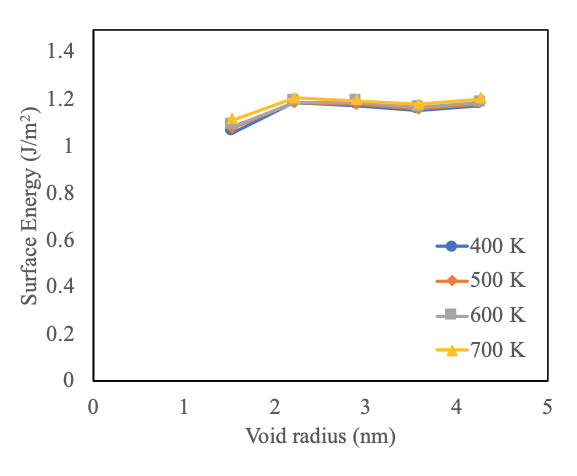
\includegraphics[width=0.6\textwidth]{1_void_Esurf.png} 
 \caption{Void surface energy as a function of radius for voids in U-10Mo from 400 K to 700 K.}
 \label{fig:voidE}
\end{figure}

An example bubble is shown in Fig. \ref{fig:bubex}. Atoms are progressively inserted into a void, leading to an increasing Xe to vacancy ratio as a function of simulation time, resulting in a highly pressurized Xe bubble at the end of the simulation. The maximum Xe/vacancy ratio obtained is approximately 0.5, which was observed to be sufficiently high to obtain a bubble pressure of a few GPa, which ensures investigation of all likely bubble pressures in these systems. 


\begin{figure}[h]
 \centering
 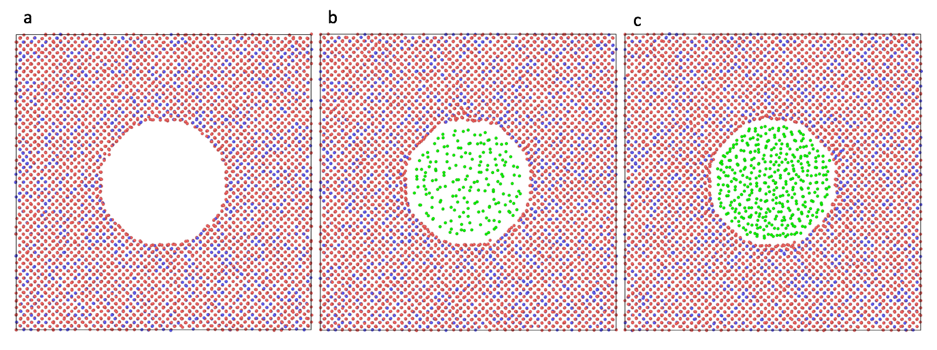
\includegraphics[width=1.0\textwidth]{2_bubex.png} 
 \caption{A Xe bubble at 500 K with a diameter of 7.1 nm in U-10Mo as a function of time. Starting from a void (a), to a Xe/vacancy ratio of 0.16 (b), and a Xe/vacancy ratio of 0.32 (c). Red atoms are U, blue atoms are Mo and green atoms are Xe. }
 \label{fig:bubex}
\end{figure}

\FloatBarrier

The bubble formation energy can be calculated by the following equation:

\begin{equation}
\label{eq:bubE}
E_f^{bub}= E^{bub}-\frac{N^{void}}{N^{sys}}E^{sys}
\end{equation}

where E$^{bub}$ is the energy of the system with a bubble, N$^{void}$ is the number of atoms in the system with a void, E$^{sys}$ is the energy of the bulk system (no voids or bubbles) and N$^{sys}$ is the number of atoms in the bulk system. The energy per atom of Xe in its reference state is neglected in this calculation, as the energy is sufficiently small ($<$ 0.01 eV/at) to result in only statistically insignificant changes to formation energies. In order to compare different bubble sizes to one another, a relative bubble energy is defined as the bubble formation energy less the void formation energy. With this formalism, only the excess energy attributable to the Xe atoms and their subsequent influence on the energy of the system is analyzed. This allows for the investigation of energetic effects of Xe bubbles for different bubble sizes. The relative bubble energy at 500 K is shown in Fig. \ref{fig:bubE} for bubbles of diameter 3.1, 4.4, 5.8, 7.1 and 8.5 nm. 

\begin{figure}[h]
 \centering
 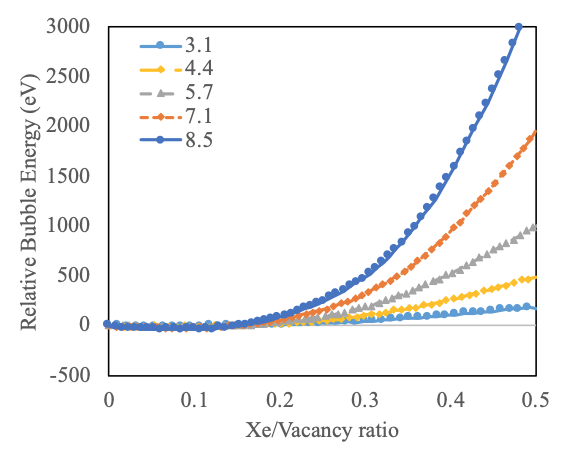
\includegraphics[width=0.6\textwidth]{3_bubE.png} 
 \caption{Relative bubble energy at 500 K as a function of Xe/vacancy ratio for bubbles of five unique sizes. Bubble diameters labeled, units in nm.}
 \label{fig:bubE}
\end{figure}

For all bubbles, there is a region below a Xe/vacancy ratio of 0.15 where additional Xe atoms inserted into the bubble produce no noticeable change in the relative bubble energy\DIFaddbegin \DIFadd{, which corresponds to a Xe molar volume of approximately 80 cm$^3$/mol }\DIFaddend . There can even exist a slight reduction in system energy due to Xe aiding in the faceting of the low pressure bubble. Above a Xe/vacancy ratio of approximately 0.15, the relative bubble energy displays a quadratic increase as a function of the Xe/vacancy ratio. The specific nature of the quadratic growth is dependent upon the bubble size, where a larger bubble displays a more rapid increase in relative bubble energy. This shows that it is much more difficult to obtain a high Xe/vacancy ratio in large bubbles compared to small bubbles. 

\FloatBarrier

The energetic preference for adding or removing a Xe atom into an existing bubble can be investigated by looking at the binding energy of the nth Xe atom in a given bubble. The binding energy of the nth Xe atom in a given bubble can be defined as:

\begin{equation}
\label{eq:bind}
E^{bind}= E(n)-E(n-1) - E_{Xe}\DIFdelbegin \DIFdel{$^{Sub-Vac}$
}\DIFdelend \DIFaddbegin \DIFadd{^{Sub} + E_{Vac}
}\DIFaddend \end{equation}

where E(n) is the energy of a system with a bubble with n Xe atoms, E(n-1) is the energy of system with a bubble with n-1 Xe atoms\DIFdelbegin \DIFdel{and E$_{Xe}^{Sub-Vac}$ is the energy difference between a Xe subtitutional-vacancy pair and a divacancy. The }\DIFdelend \DIFaddbegin \DIFadd{, E$_{Xe}^{Sub}$ is the formation energy of a Xe substitutional, and E$_{Vac}$ is the formation energy of a monovacancy. The addition of a vacancy indicates the two systems of comparison with a fixed bubble size: 1) a bubble with $m$ vacancies and $n-1$ Xe, and a substitutional Xe atom, 2) a bubble with $m$ vacancies and $n$ Xe, and a monovacancy in the lattice. The Xe substitutional reference state was chosen as this is the low energy defect configuration for Xe in U-10Mo. This was the assumed configuration based on density functional theory calculations in pure bcc U \cite{beelerASTM}. However, specific calculations utilizing the interatomic potential were undertaken to verify this information. A simulation supercell of 1024 atoms (8x8x8 unit cells) was utilized to calculate the energy, at 400 K, of bcc U, bcc Mo and bcc U-10Mo. Due to the large number of possible unique configurations of a random solid substitutional alloy, one thousand unique simulations were performed to calculate the energies of alloy systems and ensure converged energies. The }\DIFaddend formation energy of a \DIFaddbegin \DIFadd{U-10Mo alloy was found to be 0.18 eV/at. Point defects investigated included vacancy, interstitial, divacancy, Xe substitutional, Xe interstitial and a }\DIFaddend Xe \DIFdelbegin \DIFdel{sub-vac defect is determined to be 5.2 eV. This is a likely isolated Xe defect complex, as this defectstructure is lower in energy than a Xe interstitial (6.2 eV) or a Xe }\DIFdelend \DIFaddbegin \DIFadd{substitutional-vacancy pair. To account for the non-zero formation energy in point defect calculations, equation \ref{eq:eform} was utilized, 
}

\begin{equation}
\DIFadd{\label{eq:eform}
E_f^{def}= E_F^{def} - E_F^{alloy} 
}\end{equation}

\DIFadd{where E$_F^{alloy}$ is the total formation energy of an alloy of U-Mo, and E$_F^{def}$ is the total formation energy of a U-Mo alloy with a defect. Each of these total formation energies are calculated via equation \ref{eq:eftot}
}

\begin{equation}
\DIFadd{\label{eq:eftot}
E_F= E_{Tot} - E_U\times N_U - E_{Mo}\times N_{Mo}  
}\end{equation}

\DIFadd{where E$_{Tot}$ is the total energy of the system, E$_U$ is the energy per atom of bcc U, E$_{Mo}$ is the energy per atom of bcc Mo, and N$_U$ and N$_{Mo}$ are the number of U and Mo atoms in the system of interest, respectively. Subsequently, the E$_f^{def}$, which is the individual defect formation energy, can be calculated. The subsequent defect formation energies are presented in Table \ref{tab:defects}. 
}

\begin{table}[h!]
\caption{\DIFaddFL{Point defect formation energies and binding energies in U-10Mo at 400 K. Units in eV. }}
\label{tab:defects}
\begin{center}
\begin{tabular}{|c|c|c|}
     \hline
\DIFaddFL{Defect Type }& \DIFaddFL{Formation Energy }& \DIFaddFL{Binding Energy  }\\
\hline
\DIFaddFL{Vacancy }& \DIFaddFL{1.6 }& \DIFaddFL{-  }\\
\DIFaddFL{Interstitial }& \DIFaddFL{1.1 }& \DIFaddFL{- }\\
\DIFaddFL{Xe }\DIFaddendFL substitutional \DIFdelbeginFL \DIFdelFL{(5.6 eV). When a Xe is removed from this }\DIFdelendFL \DIFaddbeginFL & \DIFaddFL{6.1 }& \DIFaddFL{- }\\
\DIFaddFL{Divacancy }& \DIFaddFL{2.1 }& \DIFaddFL{-1.2 }\\
\DIFaddendFL Xe sub-vac \DIFdelbeginFL \DIFdelFL{defect, there exists a residual divacancy (1.2 eV), hence utilizing the energy difference between the Xe sub-vac and a divacancy in the binding energy calculation.
}\DIFdelendFL \DIFaddbeginFL \DIFaddFL{pair }& \DIFaddFL{7.4 }& \DIFaddFL{-0.4  }\\
     \hline
\end{tabular}
\end{center}
\label{default}
\end{table}%DIF > 

\DIFadd{It should be noted that all defects are an average of both species, for example an interstitial could be either U or Mo, and this is an average over all 1000 unique simulations. The vacancy and interstitial defect energies are qualitatively coherent, based on what one would expect in bcc U \cite{beeler2010}, with a comparatively lower interstitial formation energy. The Xe substitutional energy is 6.1 eV. The Xe interstitial energy is omitted from this table, as it was observed that Xe interstitials transformed into a Xe substitutional and a matrix interstitial. There exists strong binding between individual vacancies (negative binding energy indicating attraction here) as well as a strong binding between Xe substitutionals and vacancies. The value of 6.1 eV for a Xe substitutional was utilized in equation \ref{eq:bind}.
}

\DIFaddend The binding energy of the nth Xe atom in a given bubble is shown in Fig. \ref{fig:binding}, for all bubble sizes investigated. It can be seen that the binding energy is negative for all Xe/vacancy ratios included in this study, illustrating that it is always favorable for a Xe atom to reside in a bubble, regardless of existing Xe/vacancy ratio, rather than to reside in the bulk U-Mo alloy. The binding energy does grow less strong with increasing Xe/Vac ratio, as would be expected, but there is no observed scenario where it is energetically favorable for a Xe atom to reside in the bulk instead of as an atom in the bubble. Extrapolating a quadratic fit to a binding energy of zero yields a Xe/Vac ratio of \DIFdelbegin \DIFdel{0.92}\DIFdelend \DIFaddbegin \DIFadd{0.94}\DIFaddend , where it would be energetically unfavorable for a Xe atom to reside within the bubble. However, it is very likely that as Xe/Vac ratio increases, lattice deformation around the bubble will become dramatic, altering the binding energy behavior as a function of Xe content. It should also be noted that data for all bubble sizes is included in this graph as there is no observable difference in Xe binding energy as a function of Xe/Vac ratio for different bubble sizes. 

\begin{figure}[h]
 \centering
 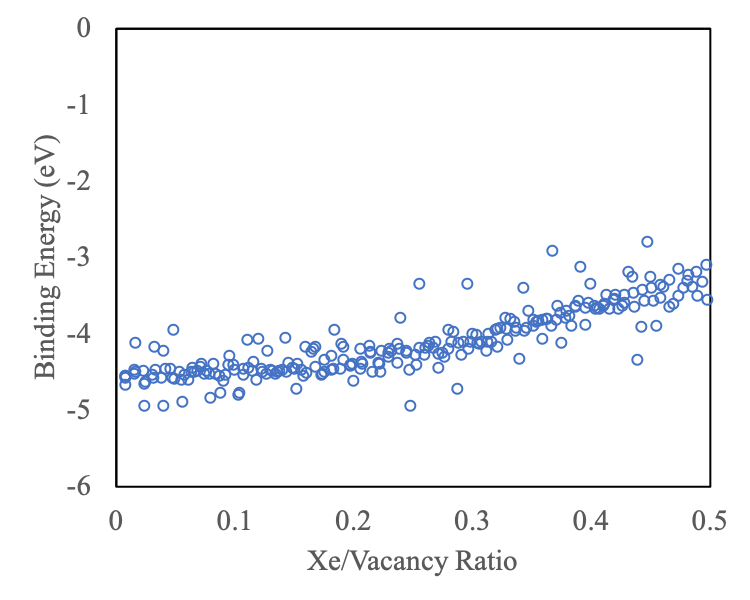
\includegraphics[width=0.6\textwidth]{4_binding.png} 
 \caption{Binding energy of the nth Xe atom in a bubble as a function of the Xe/vacancy ratio.}
 \label{fig:binding}
\end{figure}

\FloatBarrier

\subsection{Bubble pressurization transition}

In order to determine the under- to over-pressurized transition, simulations in an NPT ensemble at 400 K are performed to allow the volume to change as a function of time. The equilibrium volume of a U-10Mo alloy is determined prior to the introduction of a void and subsequent introduction of Xe atoms. A relaxed system with a void exhibits a reduced volume compared to the equilibrium system. As Xe is introduced into the void/bubble, the Xe exerts an outward force on the system. As progressively more Xe is added into the bubble, the pressure becomes significant enough to expand the bulk system and increase the supercell volume. This work defines the transition from under- to over-pressurized bubbles as the point where the volume of the system with a Xe bubble is equal to the equilibrium volume of a system with no void or bubble. Thus, at a lower than equilibrium Xe/vacancy ratio the system will have a slightly lower volume than the equilibrium system, and at a higher than equilibrium Xe/vacancy ratio the system will have a slightly higher volume than the equilibrium system. The results are shown in Fig. \ref{fig:delV}. The system becomes over-pressurized at different Xe/vacancy ratios depending upon the bubble diameter. For smaller bubbles, the transition occurs at a lower Xe/vacancy ratio. However, for the bubbles investigated, the range of variance for all bubble sizes is somewhat small. The transition occurs as early as a 0.13 Xe/vacancy ratio for a bubble of diameter 3.1 nm, and as late as a 0.20 Xe/vacancy ratio for a bubble of diameter 8.5 nm. Proceeding the transition, the volume increase is related to the size of the bubble as well, as larger bubbles see significantly more rapid volume increase with a given increase in the Xe/vacancy ratio. \DIFaddbegin \DIFadd{The quantitative value of the relative volume as a function of Xe/vacancy ratio will change with changes in supercell size volume, but the qualitative relationships will not vary. Supercell size effects were investigated in limited cases to ensure the qualitative relationships held and that the transition point was converged. 
}\DIFaddend 

\begin{figure}[h]
 \centering
 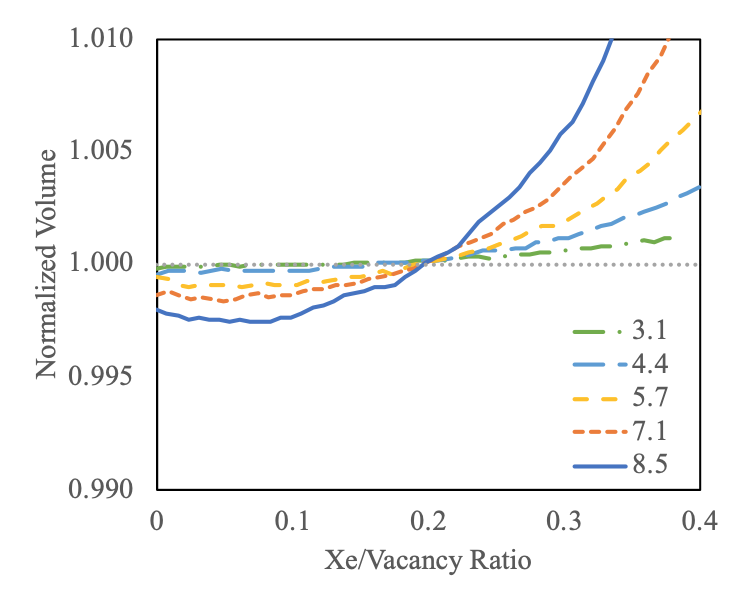
\includegraphics[width=0.6\textwidth]{5_delV.png} 
 \caption{The normalized volume of a system with a bubble as a function of Xe/vacancy ratio for five unique bubble sizes. Bubble diameters labeled, units in nm.}
 \label{fig:delV}
\end{figure}

An equilibrium bubble can be understood as the bubble existing at the under- to over-pressurized transition. Typically the pressure of such a bubble is determined by satisfying the Young-Laplace equation, often denoted by equation \ref{eq:Y-L},

\begin{equation}
\label{eq:Y-L}
P = \frac{2\gamma}{R}
\end{equation}

where $\gamma$ is the surface energy and R is the radius of the bubble. Although the Young-Laplace equation was formulated to describe the interface across fluids, it is commonly used to describe gas bubbles in solids. To verify if the Young-Laplace relationship holds for Xe bubbles in U-Mo, the predicted equilibrium pressure from \ref{eq:Y-L} is determined and compared to the computationally calculated equilibrium pressure using the Xe/vacancy ratio from Fig. \ref{fig:delV} where the normalized volume is 1. Interestingly, the results do not agree particularly well. The difference in the predicted versus calculated pressures as a function of bubble diameter is shown in Table \ref{tab:press_diff}. The difference in predicted versus calculated is most pronounced for small bubbles, however this difference is reduced as the bubble size increases. For all bubble sizes, the predicted pressure is greater than the calculated pressure. Thus, it is possible that the Young-Laplace equation does not hold for bubbles less than 10 nm in diameter in this system, however, it may apply for bubbles larger than 10 nm in diameter. 

\begin{table}[h!]
\caption{Predicted pressure based on Eq. \ref{eq:Y-L}, calculated pressure, and the subsequent difference. Units of pressure in GPa. }
\label{tab:press_diff}
\begin{center}
\begin{tabular}{|c|c|c|c|}
     \hline
Diameter (nm) & Predicted & Calculated & Difference \\
\hline
3.1 & 1.39 & 0.24 & 1.15 \\
4.4 & 1.07 & 0.31 & 0.77 \\
5.7 & 0.82 & 0.43 & 0.38 \\
7.1 & 0.65 & 0.43 & 0.22 \\
8.5 & 0.55 & 0.43 & 0.13 \\
     \hline
\end{tabular}
\end{center}
\label{default}
\end{table}%

To verify this hypothesis, two larger bubbles were investigated to determine if the predicted and calculated equilibrium pressures converged as bubble size increases. In order to accommodate larger bubbles, a larger supercell (60x60x60, 432,000 atoms) is utilized. Bubbles with a 11.2 nm diameter and a 12.6 nm diameter are investigated in an NPT ensemble at 0 pressure and 400 K, with a comparable Xe/vacancy ratio rate of change to the previous bubbles included in this study. The results of this work are included in Fig. \ref{fig:press_diff}. As the bubble radius increases, the difference between predicted and calculated pressure continues to decrease, with each pressure converging to an identical value for large bubbles. An exponential function is fit to this data, (with an R$^2$ value of 0.96), which shows that as bubble radius increases, the discrepancy between predicted and calculated equilibrium pressure exponentially decays. Given this information, we propose a modification to the Young-Laplace equation specifically for Xe bubbles in U-Mo, although this relationship may hold for other gas bubbles in other material systems. The equilibrium pressure as a function of bubble radius should be defined by equation \ref{eq:Y-Lm}

\begin{figure}[h]
 \centering
 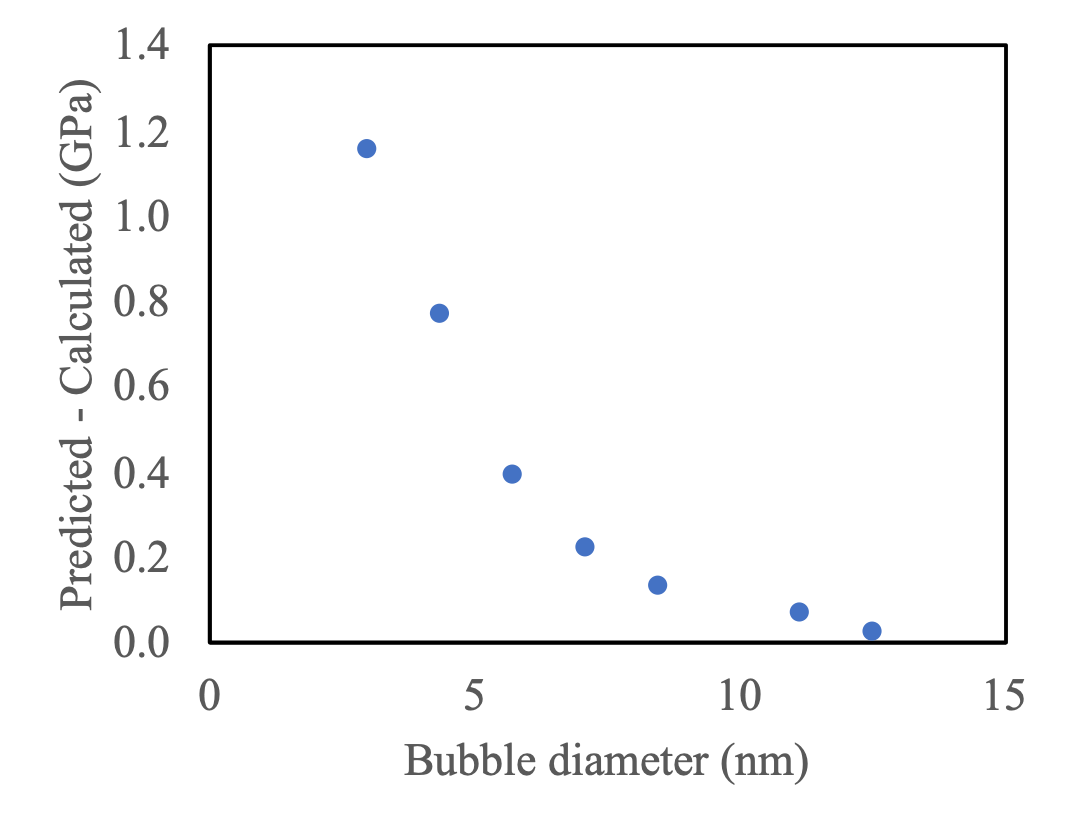
\includegraphics[width=0.6\textwidth]{6_press_diff.png} 
 \caption{\DIFdelbeginFL \DIFdelFL{Caption}\DIFdelendFL \DIFaddbeginFL \DIFaddFL{Predicted bubble pressure from Eq}\DIFaddendFL . \DIFaddbeginFL \DIFaddFL{\ref{eq:Y-L} minus the calculated pressure from molecular dynamics as a function of bubble size.}\DIFaddendFL }
 \label{fig:press_diff}
\end{figure}

\begin{equation}
\label{eq:Y-Lm}
P = \frac{2\gamma}{R} - A \times exp(-B\times R)
\end{equation}

where $\gamma$ equal 1.2 J/m$^2$ (from Fig. \ref{fig:voidE}), A equals 4.94 and B equals -0.87 for the U-Mo-Xe system. This equation decays to the Young-Laplace equation for bubble radii greater than 6 nm. It should be emphasized that this equation was not fit to data for bubbles smaller than 3 nm in diameter, and as such the authors make no conclusions regarding the validity of this expression for smaller bubbles. Additionally, it is possible that there exists a temperature dependence of this function, but since the surface energy does not vary over the temperature range of interest, it is assumed that the relationship denoted in equation \ref{eq:Y-Lm} shows only minimal variation.


\FloatBarrier

\subsection{Xe bubble equation of state in U-Mo}

The equation of state (EOS) can be determined by tracking the pressure inside the bubble and the bubble size as a function of the number of Xe atoms present in the bubble while the system is equilibrated in an NVT ensemble, which provides a pressure versus density relationship. This data can be fit to an EOS that provides a generalized function predicting the relationship between pressure, temperature and molar volume. In order to extend the applicability of the EOS, temperatures from 400 K to 700 K are analyzed, for all bubble sizes previously mentioned. No restrictions are imposed on the fitting parameters for each individual EOS. 

\subsubsection{Kaplun EOS}\label{kapluneos}

An EOS for Xe bubbles is taken from Kaplun \cite{kaplun2003}, which was also utilized in the work of Hu \cite{hu2017}, 

\begin{equation}
\label{eq:EOS}
P=\frac{RT}{v}\bigg( 1+\frac{c}{v-b}\bigg)-\frac{a}{v^2}
\end{equation}

where \textit{R} is the gas constant for Xe (8.314 J/mol-K\cite{kaplun2003}), \textit{T} is the temperature in K, \textit{P} is the pressure in MPa, \textit{v} is the molar volume in cm$^3$/mol, and \textit{a}, \textit{b}, and \textit{c} are fitting parameters. This EOS reduces to the well known Van der Waals EOS when \textit{b}=\textit{c}. It appears that Hu \cite{hu2017} mislabeled the fitting parameters in their equation, according to the units of the parameters. Hu, et al. have confirmed that the correct EOS parameters from their work are \textit{a}=259,780 J-cm$^3$/mol$^2$, \textit{b}=18.928 cm$^3$/mol and \textit{c}= 280.658 cm$^3$/mol \cite{hu2017}. These parameters are utilized as the starting guess for the fitting procedure in this work to obtain an optimized EOS. 

The subsequent fit, with and without molecular dynamics data, is shown in Fig. \ref{fig:xe_eosK}. An inlay is included for molar volumes from 20 to 100 cc/mol, to better illustrate the high pressure data. The data heavily overlaps and only shows minor differences as a function of temperature and as such the individual isotherms are difficult to distinguish. For clarity, the MD data is removed in Fig. \ref{fig:xe_eosK}b. and the optimized EOS is displayed on a log/linear scale to emphasize the differences between the individual isotherms. The optimized coefficients for the equation of state are \textit{a}=-870912.08 J-cm$^3$/mol$^2$, \textit{b}=27.133 cm$^3$/mol, \textit{c}=88.987 cm$^3$/mol. Compared to the work of Hu, this is a significant decrease in the parameter \textit{a}, a slightly larger value in \textit{b}, and a substantial decrease in \textit{c}. \DIFdelbegin \DIFdel{Emphasis }\DIFdelend \DIFaddbegin \DIFadd{Although the work of Hu utilized the same interatomic potential as this work, the area of interest with regard to bubble properties was dramatically different. Hu investigated small bubbles, less than 2 nm in diameter, at high pressures, greater than 2 GPa and up to 8 GPa. They did not include bubbles with larger radii or low density Xe gas in their fitting.  As such, it is expected that there would exist differences in the results for a fitted EOS. 
}

\DIFadd{Considering the fitted parameters, emphasis }\DIFaddend should be drawn to the negative magnitude of the \textit{a} parameter. In the original Van der Waals formalism, the \textit{a/v$^2$} term was included to provide for intermolecular attraction. Typical values of \textit{a} are positive \cite{kaplun2003}, indicating net attraction between molecules and a reduction in the overall pressure. However, in this study, the \textit{a} parameter is negative, indicating additional repulsion leading to an increase in the pressure of the system. This could potentially be due to the fact that these are generally high pressure systems, or this could be an aspect of the interaction of the Xe gas with the U-Mo matrix. Kaplun states that their derivation of a modified Van der Walls EOS loses applicability in regimes of high pressure and density, and they only compare to Xe pressures of 5 MPa and below, which would be considered extremely low for this work. Regardless, at very low gas densities, the \textit{a/v$^2$} term vanishes and this equation converges to the ideal gas law. Thus, although the magnitude of \textit{a} is atypical for isolated gases, it is deemed representative of high pressure Xe bubbles in U-Mo in this work.

The accuracy of the EOS fit can be quantified in a number of ways. A root-mean squared deviation (RMSD) is likely not the best metric, due to the large range of pressures in the data set covering multiple orders of magnitude. Thus, it can be better to gauge accuracy via a normalized RMSD (NRMSD), which is defined by dividing the RMSD by the range (the difference of the maximum and minimum) of the dataset, or via a total relative error, which is the summation of the relative error of each individual data point divided by the total number of data points. Both metrics will be used here, with emphasis placed on total relative error. The NRMSD of the optimized Kaplun EOS compared to the MD data is 6.5\% and the total relative error is 10.3\%. Considering that the pressure in this dataset varies over 3 orders of magnitude and the temperature varies over 300 K, this is considered excellent agreement. The NRMSD of the previously optimized EOS from Hu calculated with respect to the MD data in this work is 9.8\% and the total relative error is 16.5\%. Thus, using the relative error as the standard measure of accuracy, this represents approximately a 6\% improvement over the most finely calibrated EOS for Xe bubbles in U-Mo in the literature, as well as a dramatic expansion on the range of applicability, with respect to bubble size, pressure and temperature. 

\begin{figure}[h]
 \centering
 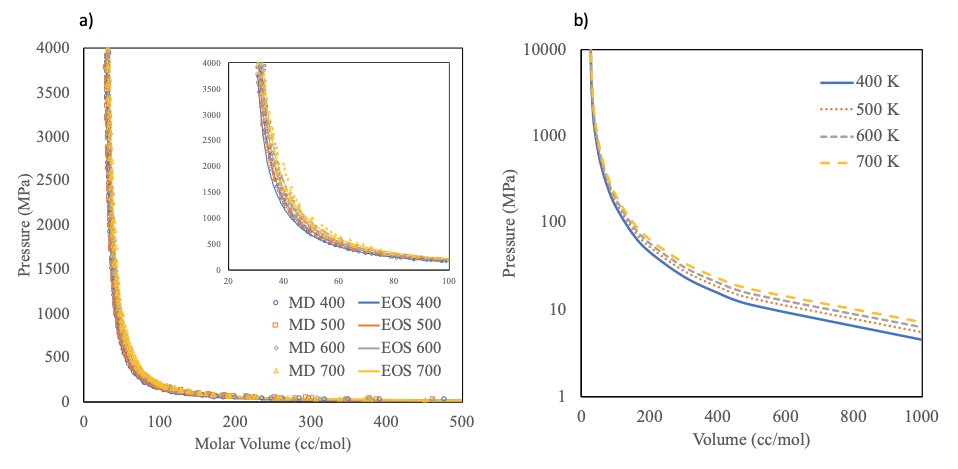
\includegraphics[width=0.8\textwidth]{7_xe_eosK.png} 
 \caption{An equation of state (EOS) based on a modified Van der Waals equation from Kaplun for Xe bubbles in U-10Mo from 400 K to 700 K (a) compared to molecular dynamics data and (b) without molecular dynamics data. }
 \label{fig:xe_eosK}
\end{figure}


\subsubsection{Virial EOS}

Due to the atypical nature of the \textit{a} parameter in \ref{kapluneos}, an additional equation of state formalism was utilized to investigate the possibility of alternate functional forms better representing the molecular dynamics data. A virial equation of state is utilized, expanded to the third order with respect to volume and the second order with respect to temperature, as is shown in equation \ref{eq:virial}, 

\begin{equation}
\label{eq:virial}
P=\frac{RT}{v}\bigg( A + \frac{B}{v} + \frac{C}{v^2} + \frac{D}{v^3}  \bigg)
\end{equation}

where \textit{A}=1, and \textit{B}, \textit{C} and \textit{D} are temperature dependent Taylor series of 1/T (\textit{B=b$_0$ + b$_1$/T + b$_2$/T$^2$}, \textit{C=c$_0$ + c$_1$/T + c$_2$/T$^2$} and \textit{D=d$_0$ + d$_1$/T + d$_2$/T$^2$}), leading to nine unique fitting parameters. The virial equation is a general function relating pressure, molar volume and temperature that can be directly derived from statistical mechanics \cite{virial}. 

The subsequent fit, with and without molecular dynamics data, is shown in Fig. \ref{fig:xe_eosV}. An inlay is included for molar volumes from 20 to 100 cc/mol. The MD data is removed in Fig. \ref{fig:xe_eosV}b. and the optimized EOS is displayed on a log/linear scale to emphasize the differences between the individual isotherms. The optimized coefficients are shown in Table \ref{tab:virial}. The NRMSD of the optimized Virial EOS compared to the MD data is 5.7\% and the total relative error is 9.0\%. This is an increase in accuracy over the modified Van der Waals EOS from this work by 1.3\% and from Hu by 7.5\%, utilizing total relative error to judge accuracy. Thus, the virial EOS provides the most accurate description of molecular dynamics information in this work and is put forth as the most accurate EOS available for description of Xe bubbles in U-Mo over this temperature and pressure range. However, comparable accuracy is achieved with the modified Van der Waals EOS and the reader is encouraged to utilize their preferred functional form. 

\begin{figure}[h]
 \centering
 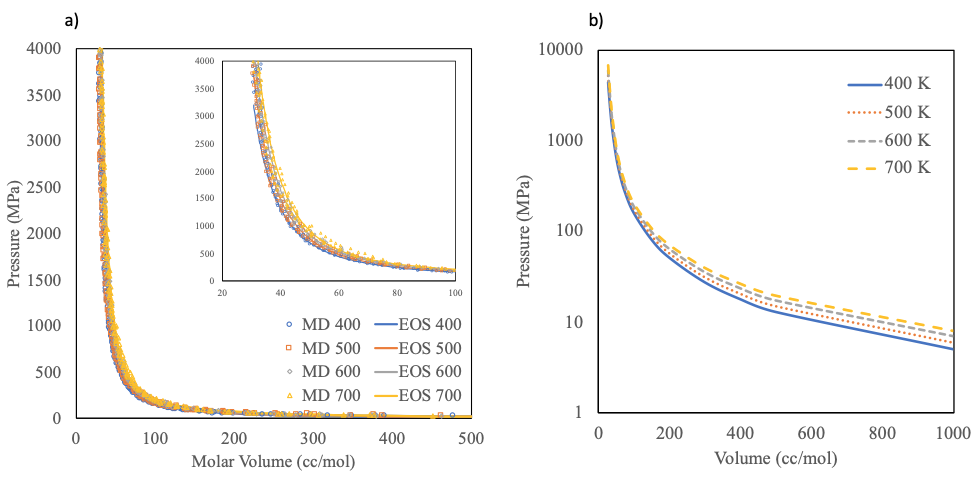
\includegraphics[width=0.8\textwidth]{8_xe_eosV.png} 
 \caption{An equation of state (EOS) based on a virial expansion for Xe bubbles in U-10Mo from 400 K to 700 K (a) compared to molecular dynamics data and (b) without molecular dynamics data. }
 \label{fig:xe_eosV}
\end{figure}

\begin{table}[h!]
\caption{Virial equation of state (Eq. \ref{eq:virial}) parameters for Xe bubbles in U-Mo.}
\label{tab:virial}
\begin{center}
\begin{tabular}{|c|c|}
     \hline
      Parameter & Value \\
     \hline
     \textit{b$_0$} & 197.229 cm$^3$/mol \\
     \textit{b$_1$} & 120307.145 cm$^3$-K/mol  \\
     \textit{b$_2$} & 60.555 cm$^3$-K$^2$/mol \\
     \textit{c$_0$} & -22038.723 cm$^6$/mol$^2$ \\
     \textit{c$_1$} & 2292.793 cm$^6$-K/mol$^2$  \\
     \textit{c$_2$} & -117.564 cm$^6$-K$^2$/mol$^2$ \\
     \textit{d$_0$} & 1030015.045 cm$^9$/mol$^3$ \\
     \textit{d$_1$} & -5.200 cm$^9$-K/mol$^3$ \\
     \textit{d$_2$} & -280.677 cm$^9$-K$^2$/mol$^3$ \\
     \hline
\end{tabular}
\end{center}
\label{default}
\end{table}%

\FloatBarrier

\section{Conclusions}

This work investigated Xe bubbles in $\gamma$U-Mo from a diameter of 3 nm up to 8.5 nm and from 400 K up to 700 K. The energetic relationship of Xe bubbles with regard to voids and Xe point defects is described. The relative energy of a bubble increases quadratically as a function of Xe/vacancy ratio, with larger bubbles exhibiting a more rapid increase in energy. The binding energy of Xe atoms is negative, indicating attraction, for all bubbles and all Xe/vacancy ratios investigated. This shows that the energy of a Xe atom in the U-Mo lattice is sufficiently high, such that Xe will always want to reside in the bubble, regardless of bubble pressure investigated in this work. The under- to over-pressurized transition for bubbles is determined. This transition is below a Xe/vacancy ratio 0.2 for all bubbles in this work. A modification of the Young-Laplace equation is suggested to determine the equilibrium volume pressure of Xe bubbles in U-Mo. Finally, two distinct equations of state were fit to the pressure as a function of molar volume and temperature for Xe in U-Mo bubbles. The virial EOS variant represents an improvement in accuracy and extended applicability compared to a previously developed EOS.

The knowledge that the Xe/vacancy ratio depends on the bubble size and optimally decreases with increasing bubble diameter is valuable, in that the assumption is typically made of a constant Xe/vacancy ratio, regardless of bubble size. Also, the examined Xe/vacancy ratios in this study are somewhat lower than the previous estimate of fission gas densities in bubbles in U-Mo, although the pressures are similar in magnitude. A modification to the Young-Laplace equation will dramatically modify the suggested equilibrium state for small fission gas bubbles. The information provided in this work regarding bubble energetics, under- to over-pressurization transition, and an updated equation of state for Xe bubble in U-10Mo can be directly utilized to improve the fidelity of mesoscale models that describe fission gas induced swelling in U-Mo fuels. 

\section{Acknowledgement}
This work was supported by the U.S. Department of Energy, Office of Material Management and Minimization, National Nuclear Security Administration, under DOE-NE Idaho Operations Office Contract DE-AC07-05ID14517. This manuscript has been authored by Battelle Energy Alliance, LLC with the U.S. Department of Energy. The publisher, by accepting the article for publication, acknowledges that the U.S. Government retains a nonexclusive, paid-up, irrevocable, worldwide license to publish or reproduce the published form of this manuscript, or allow others to do so, for U.S. Government purposes. This research made use of the resources of the High Performance Computing Center at Idaho National Laboratory, which is supported by the Office of Nuclear Energy of the U.S. Department of Energy and the Nuclear Science User Facilities.

\section{References}

\bibliography{MARMOTbib}


\end{document} 
